% ======================================================================


% Sujet du document
% Informations importantes
%
%
% Prénom Nom
% H. Dube 2019
% ======================================================================
% Ce code rassemble les efforts d'étudiants de la faculté de génie  
% de l'université de Sherbrooke afin de faire un template LaTeX moderne
% dédié à l'écriture de rapport universitaire.
% Ce document est libre d'être utilisé et modifié.
% ======================================================================

% ----------------------------------------------------
% Initialisation
% ----------------------------------------------------
\documentclass{udes_rapport} % Voir udes_rapport.cls

\begin{document}
\selectlanguage{french}

% ----------------------------------------------------
% Configurer la page titre
% ----------------------------------------------------

% Information
\faculte{Génie}
\departement{génie électrique et génie informatique}
\app{1}{Éléments de statique et de dynamique}
\professeur{M. Ahmed Khoumsi et M. Raef Cherif}
\etudiants{Hubert Dubé - dubh3401 \\ Marc Sirois - sirm2508\\ Gabriel Lavoie - lavg2007}
\dateRemise{4 septembre 2019}


% ======================================================================
\pagenumbering{roman} % met les numéros de pages en romain
% ----------------------------------------------------
% Page titre
% ----------------------------------------------------
\fairePageTitre{LOGO} % Options: [STD, LOGO]
\newpage

% ----------------------------------------------------
% Table des matières
% ----------------------------------------------------
\tableofcontents
\newpage


% ----------------------------------------------------
% Table des figures
% ----------------------------------------------------
\listoffigures
\newpage



% ======================================================================
% Document
% ======================================================================
\pagenumbering{arabic} % met des chiffres arabes
\setcounter{page}{1} % reset les numéros de pages
%%%%%%%%%%%%%%%%%%%%%%%%%%%%%%%%%%%%%%%%%%%%%%%%%%%%%%
%{Analyse du signal
%%%%%%%%%%%%%%%%%%%%%%%%%%%%%%%%%%%%%%%%%%%%%%%%%%%%%%
\section{Introduction}

\section{Cinématique}
\subsection{Mouvement de A dans le cas général}
Le positionnement de $\overrightarrow{OA}$ peut être exprimé par l'addition:
\begin{equation}
	\overrightarrow{OA} = \overrightarrow{OB} + \overrightarrow{BA}
\end{equation}
	\[	\overrightarrow{OA_x} = l_1 cos(\theta) + l_2 cos(\phi) 			\]
	\[	\overrightarrow{OA_y} = l_1 sin(\theta) + l_2 sin(\phi)			\]


la vitesse étant la dérivée de la position :
\begin{equation}
\overrightarrow{V_A} = \frac{d\overrightarrow{OA}}{dt}
\end{equation}

\[ \overrightarrow{V_Ax} = \frac{d(\overrightarrow{OA_x}}{dt} = \frac{d(l_1 cos(\theta) + l_2 cos(\phi))}{dt}	\]
\[ \overrightarrow{V_Ax} = -l_1 sin(\theta) \dot{\theta} -l_2 sin(\phi) \dot{\phi}								\]
\[ \overrightarrow{V_Ay} = \frac{d(\overrightarrow{OA_y}}{dt} = \frac{d(l_1 sin(\theta) + l_2 sin(\phi))}{dt}	\]
\[ \overrightarrow{V_Ax} = l_1 cos(\theta) \dot{\theta} -l_2 cos(\phi) \dot{\phi}								\]


La même stratégie peut être utilisé pour obtenir l'accélération :
\begin{equation}
\overrightarrow{a_A} = \frac{d\overrightarrow{V_A}}{dt}	\\
\end{equation}
\[	\overrightarrow{a_Ax} = \frac{d\overrightarrow{OA_x}}{dt} = \frac{ d(l_1 cos(\theta) + l_2 cos(\phi))}{dt}		\]
\[	\overrightarrow{a_Ay} = \frac{d\overrightarrow{OA_y}}{dt} = \frac{d(l_1 cos(\theta) + l_2 cos(\phi))}{dt}		\]

\subsection{Mouvement horizontal de A}

\noindent\begin{minipage}{\textwidth} 
\begin{minipage}{0.5\textwidth}
  \centering
  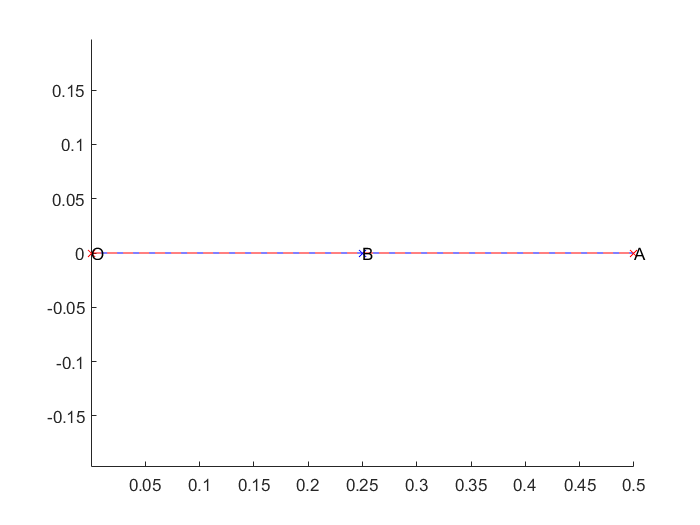
\includegraphics[width=.75\linewidth]{pos_hori_0}
  \captionof{subfigure}{Position initiale}
  \label{pos_hori:position_horizontal_initiale}
\end{minipage}%
\begin{minipage}{0.5\textwidth}
  \centering 
  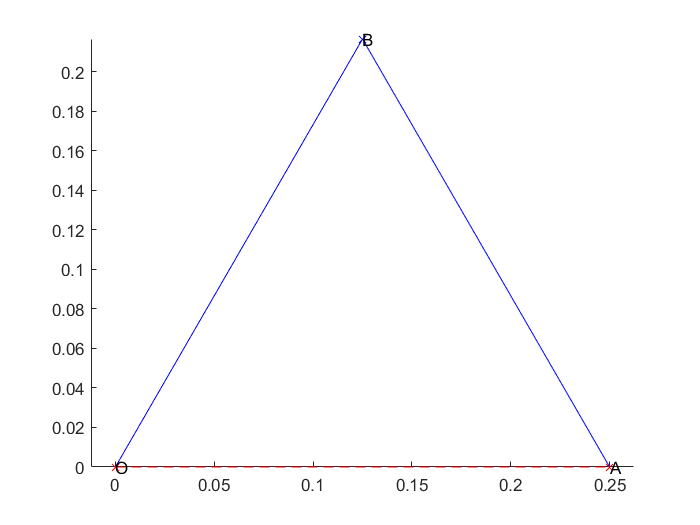
\includegraphics[width=.75\linewidth]{pos_hori_pi3} 
  \captionof{subfigure}{Position finale} 
  \label{pos_hori:position_horizontal_finale} 
\end{minipage} 
\captionof{figure}{Position du mouvement horizontale} 
\label{pos_hori} 
\end{minipage}

En position initiale, la distance entre le moteur O et le poids est de 2L. 
En position finale, la distance OA forme un triangle équilatéral avec les deux bras, puisque les trois
angles sont de pi/3

\begin{center}
	\centering
	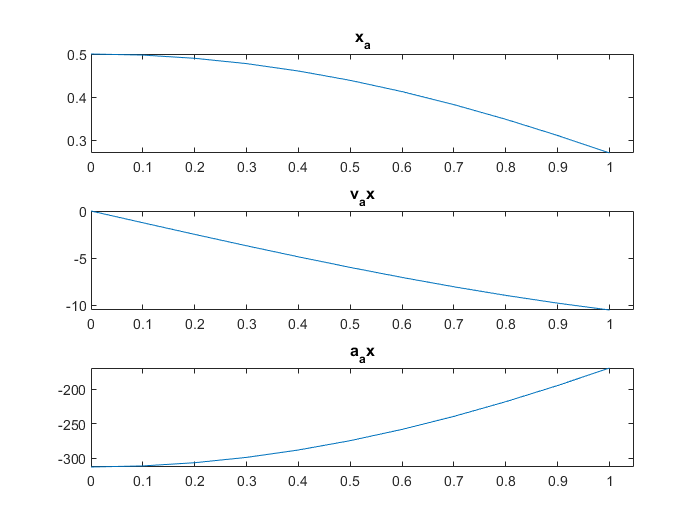
\includegraphics[width=0.7\textwidth]{theta_hori}
	\captionof{figure}{Composantes en fonction de $\protect\theta$}
	\label{composantes_horizontale_theta}
\end{center}

\subsection{Mouvement vertical de A}

\noindent\begin{minipage}{\textwidth} 
\begin{minipage}{0.5\textwidth}
  \centering
  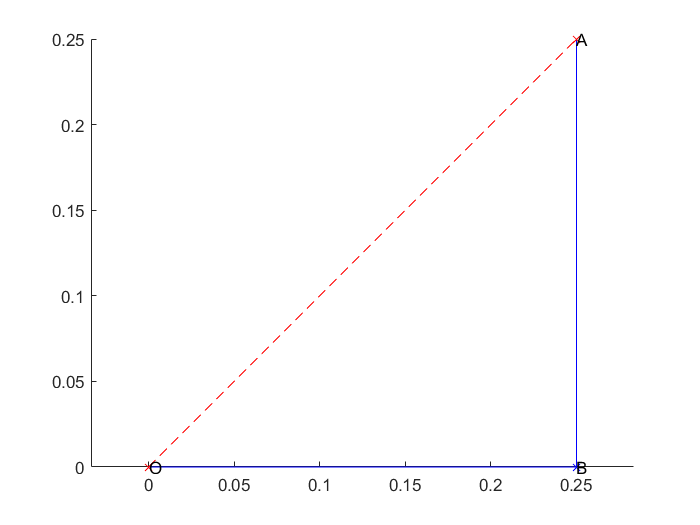
\includegraphics[width=.75\linewidth]{pos_vert_0}
  \captionof{subfigure}{Position initiale}
  \label{pos_vert:position_verticale_initiale}
\end{minipage}%
\begin{minipage}{0.5\textwidth}
  \centering 
  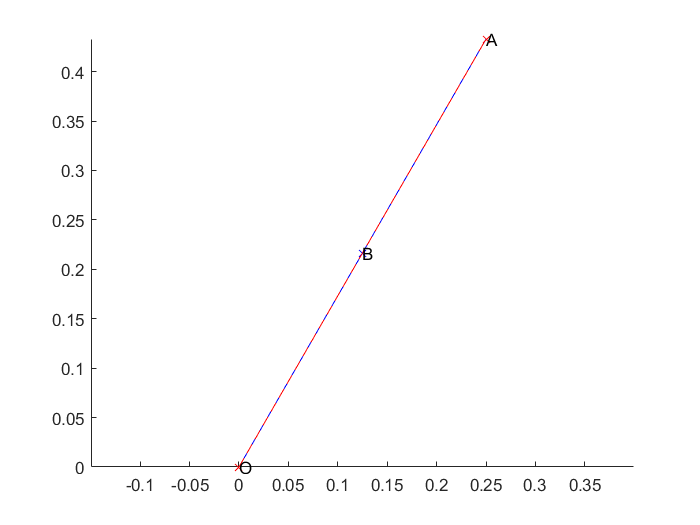
\includegraphics[width=.75\linewidth]{pos_vert_pi3} 
  \captionof{subfigure}{Position finale} 
  \label{pos_vert:position_verticale_finale} 
\end{minipage} 
\captionof{figure}{Position du mouvement vertical} 
\label{pos_vert} 
\end{minipage}

\begin{center}
	\centering
	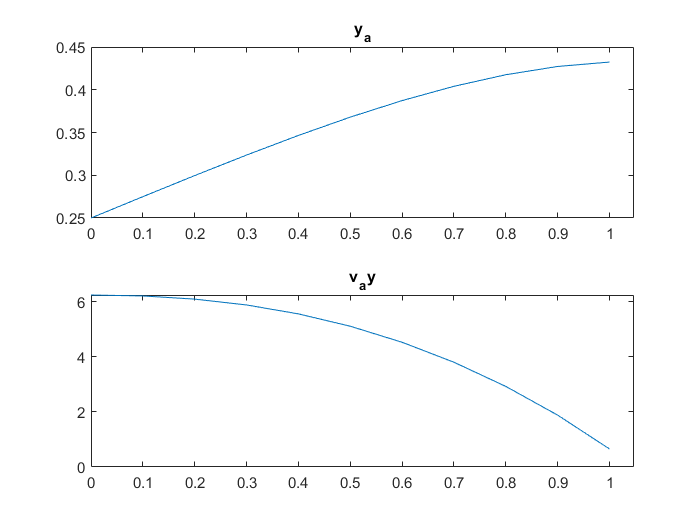
\includegraphics[width=0.7\textwidth]{theta_vert}
	\captionof{figure}{Composantes en fonction de $\protect\theta$}
	\label{composantes_verticale_theta}
\end{center}
\subsection{Analyse avec Matlab}



\section{Statique et dynamique}
\subsection{Statique}
La figure ci-dessous démontre les forces en action qui influencent le calcul de la force $F_b$ lorsque le robot est immobile.
\begin{center}
	\centering
	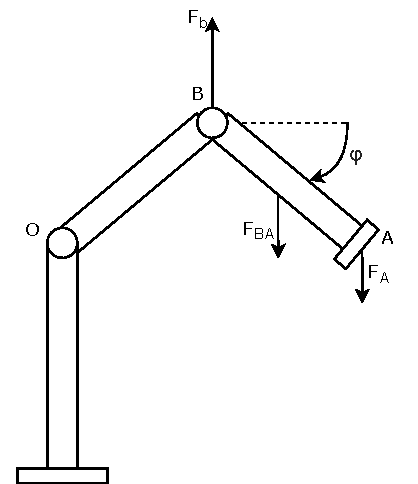
\includegraphics[width=0.3\textwidth]{statique_fb}
	\captionof{figure}{Diagramme des forces en statique pour le calcul de $F_b$}
	\label{statique_fb}
\end{center}
La somme des forces d'un système statique est égale à 0, tel que décrit par:
\begin{equation}
	\sum \overrightarrow F = \overrightarrow 0
\end{equation}
En suivant la formule et faisant la sommation des vecteurs de force, on obtient:
	\[	\sum \overrightarrow F = \overrightarrow 0 = \overrightarrow{F_b} + \overrightarrow{F_{BA}} + \overrightarrow{F_A}	\]
	\[	\begin{bmatrix}
	0\\ 
	0
	\end{bmatrix} = \begin{bmatrix}
	F_{bx}\\ 
	F_{by}
	\end{bmatrix} + \begin{bmatrix}
	0\\ 
	-F_{BA}
	\end{bmatrix} + \begin{bmatrix}
	0\\ 
	-F_A
	\end{bmatrix}	\]
On observe rapidement que le valeur de $F_{bx}$ est égale à 0 et que la valeur de $F_{by}$ correspond:
	\[	F_{by} = F_{BA} + F_A 	\]
En utilisant l'equation:
\begin{equation}
	F = m*g
\end{equation}
On obtient:
	\[	F_{by} = g*(m_{BA} + m_A)	\]
Et donc la valeur de Fb en statique, avec g étant l'accélération gravitationnelle:
	\[	F_b = \begin{bmatrix}
	0\\ 
	g*(m_{BA} + m_A)
	\end{bmatrix}	\]
La figure ci-dessous démontre les forces en action qui influencent le calcul du moment $C_b$:
\begin{center}
	\centering
	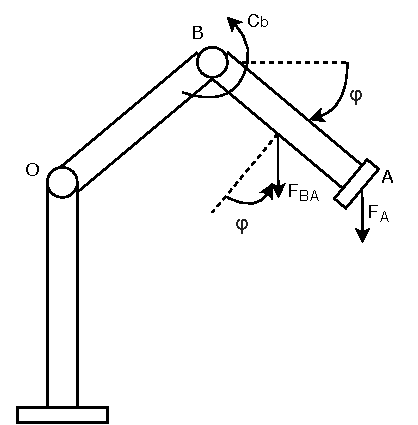
\includegraphics[width=0.3\textwidth]{statique_cb}
	\captionof{figure}{Diagramme des forces en statique pour le calcul de $C_b$}
	\label{statique_cb}
\end{center}
La somme des moments à un point (dans notre cas B) d'un système statique est égale à 0, tel que décrit par:
\begin{equation}
	\sum M_B =  0
\end{equation}
Les forces $\overrightarrow F_{BA}$ et $\overrightarrow F_A$ ont une influence tangentielle et normale à la tige BA. Pour le calcul des moments, uniquement la partie tangentielle nous intéresse (la normale n'a pas d'impact). La tangentielle se trouve à être la projection des forces ($cos\varphi$). On obtient alors:
	\[	\sum M_B =  0 = C_b - cos\varphi*F_{BA}*l_2/2 - cos\varphi*F_A*l_2	\]
En isolant $C_b$ et simplifiant l'équation avec les valeurs pour $F_{BA}$ et $F_A$ trouvées ci-haut, on obtient sa valeur pour le cas statique (avec g étant l'accélération gravitationnelle):
	\[	C_b = l_2*g*cos\varphi*(m_{BA}/2+m_A)	\]
\begin{center}
	\centering
	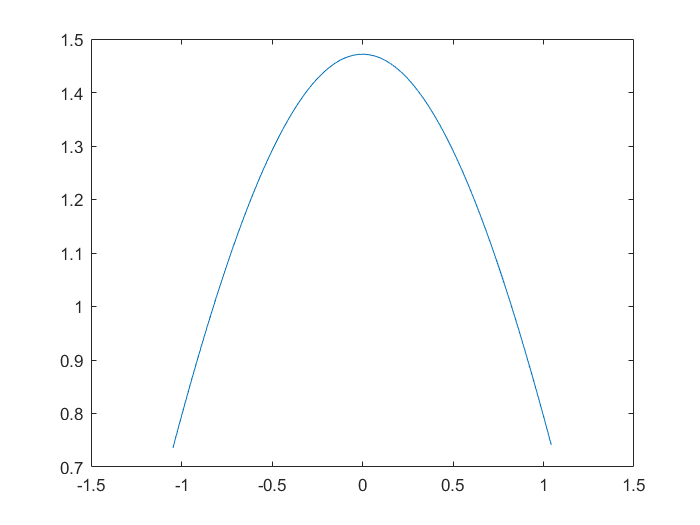
\includegraphics[width=0.7\textwidth]{couple_stat}
	\captionof{figure}{couple statique en fonction de $\protect\theta$}
	\label{couple_statique}
\end{center}
\subsection{Dynamique}
La figure ci-dessous démontre les forces en action qui influencent le calcul de la force $F_b$ lorsque le robot est immobile à l'exception de la tige BA qui a une accékération angulaire constante de $\alpha$.
\begin{center}
	\centering
	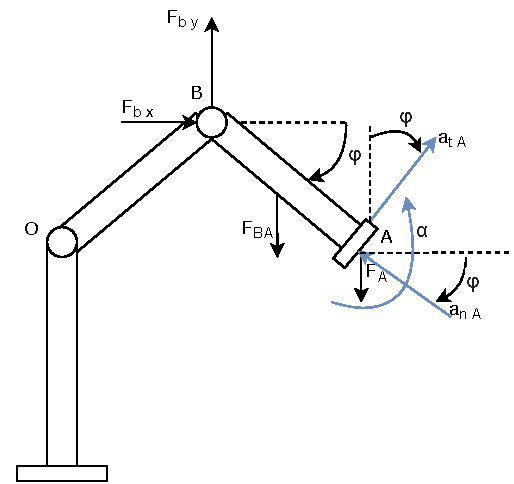
\includegraphics[width=0.3\textwidth]{dynamique_fb}
	\captionof{figure}{Diagramme des forces en dynamique pour le calcul de $F_b$}
	\label{statique_fb}
\end{center}
La somme des forces d'un système dynamique est égale à les accélérations fois les masses accélérées, tel que décrit par:
\begin{equation}
	\sum \overrightarrow F = m*\overrightarrow \gamma_G
\end{equation}
En suivant la formule et faisant la sommation des vecteurs de force, on obtient:
	\[	\sum \overrightarrow F = \overrightarrow 0 = \overrightarrow{F_b} + \overrightarrow{F_{BA}} + \overrightarrow{F_A}	\]
	\[	\begin{bmatrix}
	0\\ 
	0
	\end{bmatrix} = \begin{bmatrix}
	F_{bx}\\ 
	F_{by}
	\end{bmatrix} + \begin{bmatrix}
	0\\ 
	-F_{BA}
	\end{bmatrix} + \begin{bmatrix}
	0\\ 
	-F_A
	\end{bmatrix}	\]
On observe rapidement que le valeur de $F_{bx}$ est égale à 0 et que la valeur de $F_{by}$ correspond:
	\[	F_{by} = F_{BA} + F_A 	\]
En utilisant l'equation:
\begin{equation}
	F = m*g
\end{equation}
On obtient:
	\[	F_{by} = g*(m_{BA} + m_A)	\]
Et donc la valeur de Fb en statique, avec g étant l'accélération gravitationnelle:
	\[	F_b = \begin{bmatrix}
	0\\ 
	g*(m_{BA} + m_A)
	\end{bmatrix}	\]
\begin{center}
	\centering
	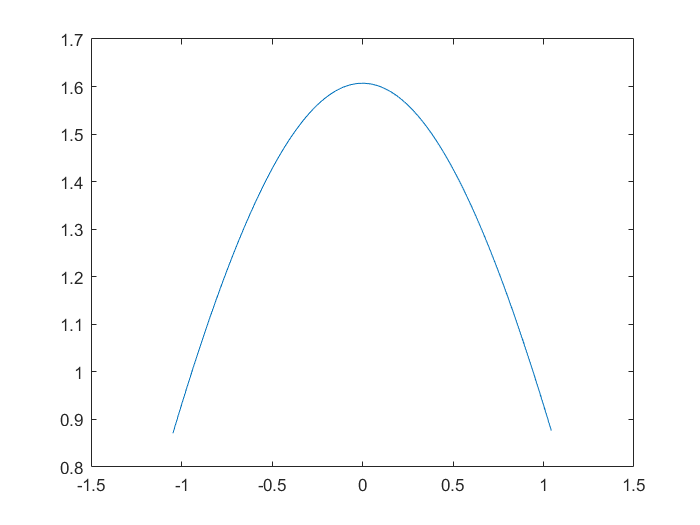
\includegraphics[width=0.7\textwidth]{couple_dyn}
	\captionof{figure}{couple dynamique en fonction de $\protect\theta$}
	\label{couple_dynamique}
\end{center}
\subsection{Analyse avec Matlab}

\section{Conclusion}

\begin{comment}
\begin{center}
	\centering
	\includegraphics[width=0.7\textwidth]{puissance}
	\captionof{figure}{Spectre de puissance d'une onde de 1kHz}
	\label{puissance}
\end{center}


\section{Filtres FIR}
\noindent\begin{minipage}{\textwidth} 
\begin{minipage}{0.5\textwidth}
  \centering
  \includegraphics[width=.75\linewidth]{ampFIR}
  \captionof{subfigure}{Amplitude}
  \label{FIR:ampFIR}
\end{minipage}%
\begin{minipage}{0.5\textwidth}
  \centering 
  \includegraphics[width=.75\linewidth]{phaseCute} 
  \captionof{subfigure}{Phase} 
  \label{FIR:phaseFIR} 
\end{minipage} 
\captionof{figure}{Filtre IIR} 
\label{FIR} 
\end{minipage}
\end{comment}

\end{document}












